%--
%-- Diagrama de Contexto
%--
\subsection{Diagrama de Contexto}

%--
%-- Agentes
%--
\subsubsection{Agentes}

\begin{enumerate}
  \item Depósito
  \item Cliente
  \item Sucursal
  \item Sistema
  \item Logística
  \item API de Logística
  \item Departamento de Stock
  \item Agente de Cobro
  \item Administrador
  \item Sistema de Correo Electrónico
  \item Financiera(API)\footnote{Ejemplo: VERAZ}
  \item Correo Argentino(API)
  \item Proveedor
\end{enumerate}
\clearpage

%--
%-- Acciones Básicas
%--
\subsubsection{Diagrama de Contexto}

\begin{figure}[H]
  \begin{center}
  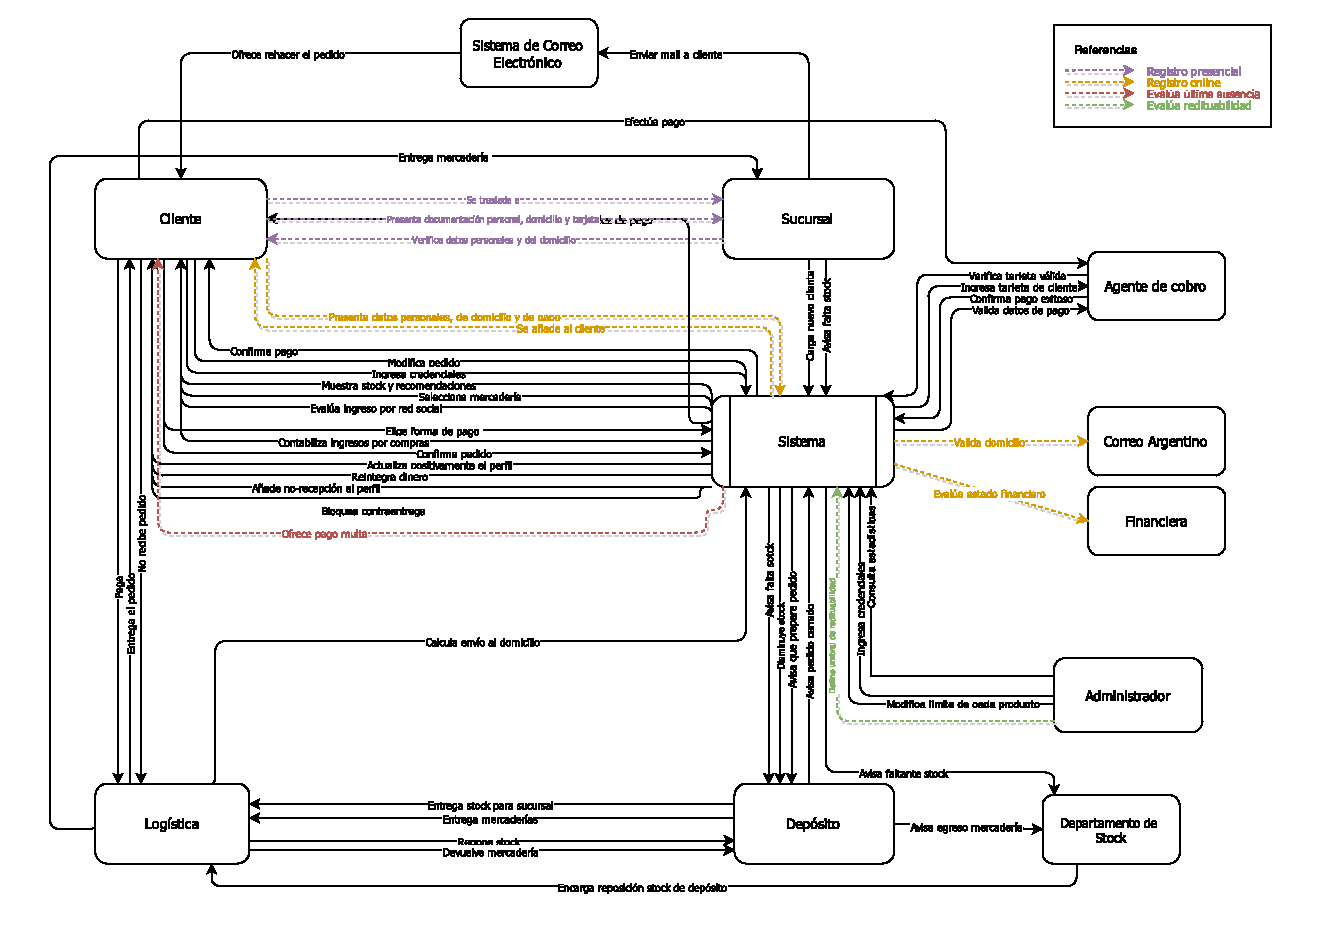
\includegraphics[height=0.65\textheight,angle=90]{tp1/images/contexto.pdf}
  \end{center}
\end{figure}
